% Intended LaTeX compiler: xelatex
\documentclass[a4paper, 12pt]{article}
\usepackage{graphicx}
\usepackage{grffile}
\usepackage{longtable}
\usepackage{wrapfig}
\usepackage{rotating}
\usepackage[normalem]{ulem}
\usepackage{amsmath}
\usepackage{textcomp}
\usepackage{amssymb}
\usepackage{capt-of}
\usepackage{hyperref}
\usepackage[danish]{babel}
\usepackage{mathtools}
\usepackage[margin=3.0cm]{geometry}
\hypersetup{colorlinks, linkcolor=black, urlcolor=blue}
\setlength{\parindent}{0em}
\parskip 1.5ex
\author{Matematik A}
\date{Vibenshus Gymnasium}
\title{Komplekse tal - Besvarelse af opgaver\\\medskip
\large Supplerende stof}
\hypersetup{
 pdfauthor={Matematik A},
 pdftitle={Komplekse tal - Besvarelse af opgaver},
 pdfkeywords={},
 pdfsubject={},
 pdfcreator={Emacs 27.2 (Org mode 9.4.4)}, 
 pdflang={Danish}}
\begin{document}

\maketitle


\section*{Opgave 1}
\label{sec:org41e9968}

Betragt de to komplekse tal \(z=3+4i\) og \(w=2-i\). Beregn og indtegn følgende sammenhænge i et Argand-diagram


\subsection*{1. \(z+w\)}
\label{sec:org3d5e69f}

Komponentform:

\begin{align*}
     z+ w &= 3+4i + 2 -i \\
     z+ w &= 3+2+ (4-1)i \\
     z+ w &= 5+ 3i 
\end{align*}

Eksponentialform:

\begin{align*}
\sqrt{5^2 + 3^2} &= 5.83095189485 \\
\tan^{-1} \left( \frac{3}{5} \right) &= 0.540419500271
\end{align*}

$$z+w= 5.83 e^{i 0.54}$$

\subsection*{2. \(w-z\)}
\label{sec:org3a96da8}

Komponentform:

\begin{align*}
    w-z &= 2 -i -(3 + 4i) \\
    w-z &= -1 -i5 
\end{align*}

Eksponentialform:

\begin{align*}
\sqrt{(-1)^2+(-5)^2} &= 5.09901951359 \\
\tan^{-1} \left( \frac{-5}{-1} \right) &= 1.373400766945016
\end{align*}

Modulus skal omskrives da det komplekse tal ligger i 3. kvadrant: \(\theta = -(\pi - 1.373)=-1.768\)

$$w-z = 5.099 e^{-1.768 i}$$


\subsection*{3. \(w \cdot z\)}
\label{sec:orgc61ce03}

Komponentform:

$$w \cdot z = (3+4i) \cdot (2-i) = 6 -i3 +8i +4 = 10+5i$$

Eksponentialform:

\begin{align*}
\sqrt{10^2+5^2} &= 11.18033988749895 \\
\tan^{-1} \left( \frac{5}{10} \right) &=0.463647609000806
\end{align*}

$$w \cdot z = 11.180 e^{i0.464}$$

\subsection*{4. \(\frac{z}{w}\)}
\label{sec:orgdccb847}

Komponentform:

\begin{align*}
    \frac{z}{w} &= \frac{3+4i}{2-i} \\
    \frac{z}{w} &= \frac{3+4i}{2-i}\cdot \frac{2+i}{2 + i} \\ 
    \frac{z}{w} &= \frac{(3+4i)\cdot(2+i)}{2^2-i^2} \\
    \frac{z}{w} &= \frac{6+11i -4}{5}  \\
    \frac{z}{w} &= \frac{2+11i }{5}  \\
    \frac{z}{w} &= \frac{2}{5}+\frac{11}{5}i   
\end{align*}

Eksponentialform:

\begin{align*}
\sqrt{\left(\frac{2}{5}\right)^2+\left(\frac{11}{5}\right)^2} &=2.23606797749979 \\
\tan^{-1} \left( \frac{11}{2} \right) &= 1.390942827002418
\end{align*}

$$\frac{z}{w} = 2.236 e^{i 1.391}$$

\subsection*{5.\(z^* \cdot w + w^*\cdot z\)}
\label{sec:org8ee4cd0}

Komponentform:

\begin{align*}
     z^* \cdot w + w^*\cdot z &= (3-4i) \cdot(2-i) + (2+i) \cdot(3+4i) \\
           z^* \cdot w + w^*\cdot z &= 6-3i -8i -4 +6+8i+3i-4 \\
           z^* \cdot w + w^*\cdot z &= 4
\end{align*}

Eksponentialform:

$$z^* \cdot w + w^* \cdot z = 4 \cdot e^{i \cdot 0}=4$$

\subsection*{6. \(w^2\)}
\label{sec:org46d0301}

Komponentform:

\begin{align*}
    w^2 &= (2-i)^2\\
    w^2 &= 2^2 + i^2 - 2 \cdot 2 \cdot i\\
    w^2 &= 4 - 1 - 4 \cdot i\\
    w^2 &= 3 - 4 \cdot i
\end{align*}

Eksponentialform:

\begin{align*}
\sqrt{3^2+4^2} &= 5.0 \\
\tan^{-1} \left( \frac{-4}{3} \right) &=- 0.9272952180016121
\end{align*}

\(w^2\) befinder sig i 4. kvadrant så vinklen stemmer overens.

$$w^2 = 5 e^{- i 0.927}$$

Alle kombinationerne for \(z\) og \(w\) kan ses på den følgende figur.

\begin{center}
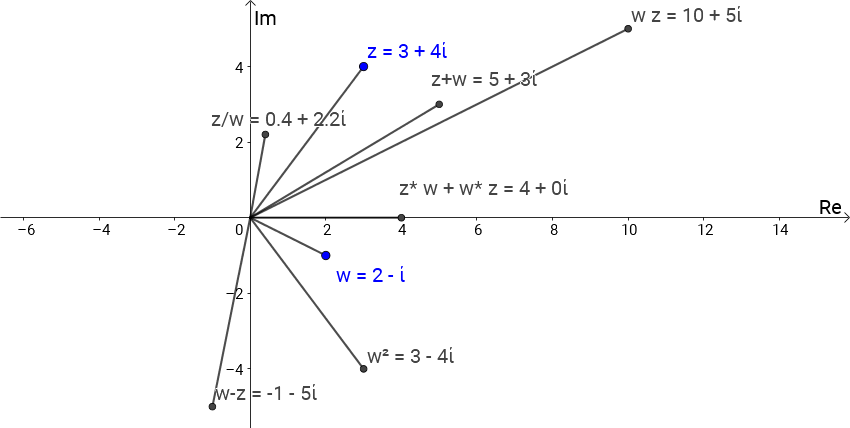
\includegraphics[width=0.8\linewidth]{./img/opgave_1.png}
\end{center}

\section*{Opgave 2}
\label{sec:org3ea0d48}

Evaluering eller simplificering af komplekse udtryk.

\subsection*{1. \(Re\left(e^{2iz}\right)\)}
\label{sec:org4cf14bf}

Husk at \(z=x+iy\)

\begin{align*}
    e^{2i z} &= e^{2i (x+iy)} = e^{2ix -2y}\\
             &= e^{2ix} \cdot e^{-2y} \\
             &= \left(\cos(2x) + i\sin(2x)\right) \cdot e^{-2y} \quad \text{ Benytter de Moivres formel} \to \\
    Re\left(e^{2iz}\right) &= Re\left(\left(\cos(2x) + i\sin(2x)\right) \cdot e^{-2y} \right) \\
    Re\left(e^{2iz}\right) &= \cos(2x) \cdot e^{-2y}  \quad \triangle
\end{align*}

\subsection*{2. \(\left(-1 + \sqrt{3} \cdot i\right)^{\frac{1}{2}}\)}
\label{sec:orgab8f00d}

Først defineres \(w=-1 +\sqrt{3} \cdot i\) således at udtrykket kan skrives som

$$w^{\frac{1}{2}}\,.$$

\(w\) skrives på polær form:

$$|w| = \sqrt{(-1)^2+\left(\sqrt{3}\right)^2} = \sqrt{4} = 2$$

$$arg(w) = tan^{-1} \left(\frac{\sqrt{3}}{-1}\right) = - \frac{\pi}{3} + \pi \cdot n, \text{ hvor $n$ er et heltal}$$

I dette tilfælde vælges \(n=1\) sa \(w\) vil ligge i 2. kvadrant. Dermed er \(arg(w) = -\frac{\pi}{3}+\pi = \frac{2\pi}{3}\).

Det oprindelige udtryk kan nu skrives som

\begin{align*}
 \left(-1 + \sqrt{3} \cdot i\right)^{\frac{1}{2}} &= \left(2 \cdot e^{i\cdot \left( \frac{2\pi}{3} \right)}\right)^{\frac{1}{2}} \\
 \left(-1 + \sqrt{3} \cdot i\right)^{\frac{1}{2}} &= \sqrt{2} \cdot e^{i\cdot  \frac{\pi}{3} } \quad \triangle
\end{align*}

\subsection*{3. \(\left \lvert e^{\left(i^\frac{1}{2}\right)}\right\rvert\)}
\label{sec:org45138d9}

\(i\) omskrives til \(i=e^{i \frac{\pi}{2}}\)

\begin{align*}
    e^{\left(i^\frac{1}{2}\right)} &= e^{\left(e^{i\frac{\pi}{2}}\right)^{\frac{1}{2}}} =e^{\left(e^{i \frac{\pi}{4}}\right)}
\end{align*}

Udnytter nu, at \(|z|^2 = z \cdot z^*\)

\begin{align*}
    \left \lvert e^{\left(i^\frac{1}{2}\right)}\right\rvert^2 &= e^{\left(e^{i \frac{\pi}{4}}\right)}\cdot e^{\left(e^{-i \frac{\pi}{4}}\right)}  \\
    \left \lvert e^{\left(i^\frac{1}{2}\right)}\right\rvert^2 &= e^{e^{i \frac{\pi}{4}}+e^{-i \frac{\pi}{4}}}  \\
    \left \lvert e^{\left(i^\frac{1}{2}\right)}\right\rvert^2 &= e^{2 \cos\left(\frac{\pi}{4}\right)}  \quad \text{ Her benyttes ligning (3.11) i kompendiet.} \\
    \left \lvert e^{\left(i^\frac{1}{2}\right)}\right\rvert &= e^{ \cos\left(\frac{\pi}{4}\right)}  \\
    \left \lvert e^{\left(i^\frac{1}{\sqrt{2}}\right)}\right\rvert &= e^{\frac{1}{\sqrt{2}}} \lor e^{-\frac{1}{\sqrt{2}}}  \quad \triangle
\end{align*}

\subsection*{4. \(e^{i^3}\)}
\label{sec:org9284bd9}

Skrives let op som

\begin{align*}
e^{i^3} &= e^{i \cdot i \cdot i} = e^{-i}\\
e^{i^3} &= \cos(-1) + i \sin(-1) \quad \text{Benytter Eulers ligning (2.18)}\\
e^{i^3} &= 0.54 - i 0.84  \quad \triangle
\end{align*}

\subsection*{5. \(Im\left(2^{i+3}\right)\)}
\label{sec:org401f617}

I første omgang omskrives \(2^{i+3}\) ved hjælp af ligning (4.3)

$$2^{i+3} = e^{(i+3) \cdot \ln(2)} = e^{i \ln(2)} \cdot e^{3 \ln(2)}=e^{i \ln(2)} \cdot \left(e^{\ln(2)}\right)^3 = e^{i\ln(2)} \cdot 2^3 =e^{i\ln(2)} \cdot 8\,.$$

Første faktor i sidste ligning omskrives ved hjælp af Eulers ligning

$$2^{i+3} = e^{i \ln(2)} \cdot 8 = \left(\cos\left(\ln(2)\right) + i \sin\left(\ln(2)\right)\right) \cdot 8 \,.$$

Nu kan den imaginære del findes:

$$Im\left(2^{i+3}\right) = Im\left( \left(\cos\left(\ln(2)\right) + i \sin\left(\ln(2)\right)\right) \cdot 8 \right) = \sin(\ln(2))\cdot 8 = 5.11\quad \triangle$$

\subsection*{6. \(z=1^i\)}
\label{sec:org3146d52}

Denne opgave løses let ved hjælp af ligning (4.3)

$$z = 1^i = e^{i \cdot \ln(1)} = e^{i \cdot 0 }= e^{0} = 1 \quad \triangle$$

\subsection*{7. \(z=i^i\)}
\label{sec:org11b6a1a}

Udnytter at \(i\) selv kan skrives som \(i=e^{i \left(\frac{\pi}{2} + 2 \pi n\right)}\)

$$z=i^i= \left(e^{i \left(\frac{\pi}{2} + 2 \pi n\right)}\right)^i = e^{i \cdot i\cdot \left( \frac{\pi}{2} + 2 \pi n\right)} = e^{-1\cdot \left( \frac{\pi}{2} + 2 \pi n\right)}=e^{-\frac{\pi}{2} - 2 \pi n}\quad \triangle$$

\section*{Opgave 3}
\label{sec:orgdac9df4}

Skitsér de dele af Argand-diagrammet hvor følgende udsagn gælder

\begin{enumerate}
\item \(|z| = 2\)
\item \(|z| < 1\)
\item \(1<|z|<2\)
\end{enumerate}

De tre udsagn kan ses på den figur \ref{opg3}.

\begin{figure}[htbp]
\centering
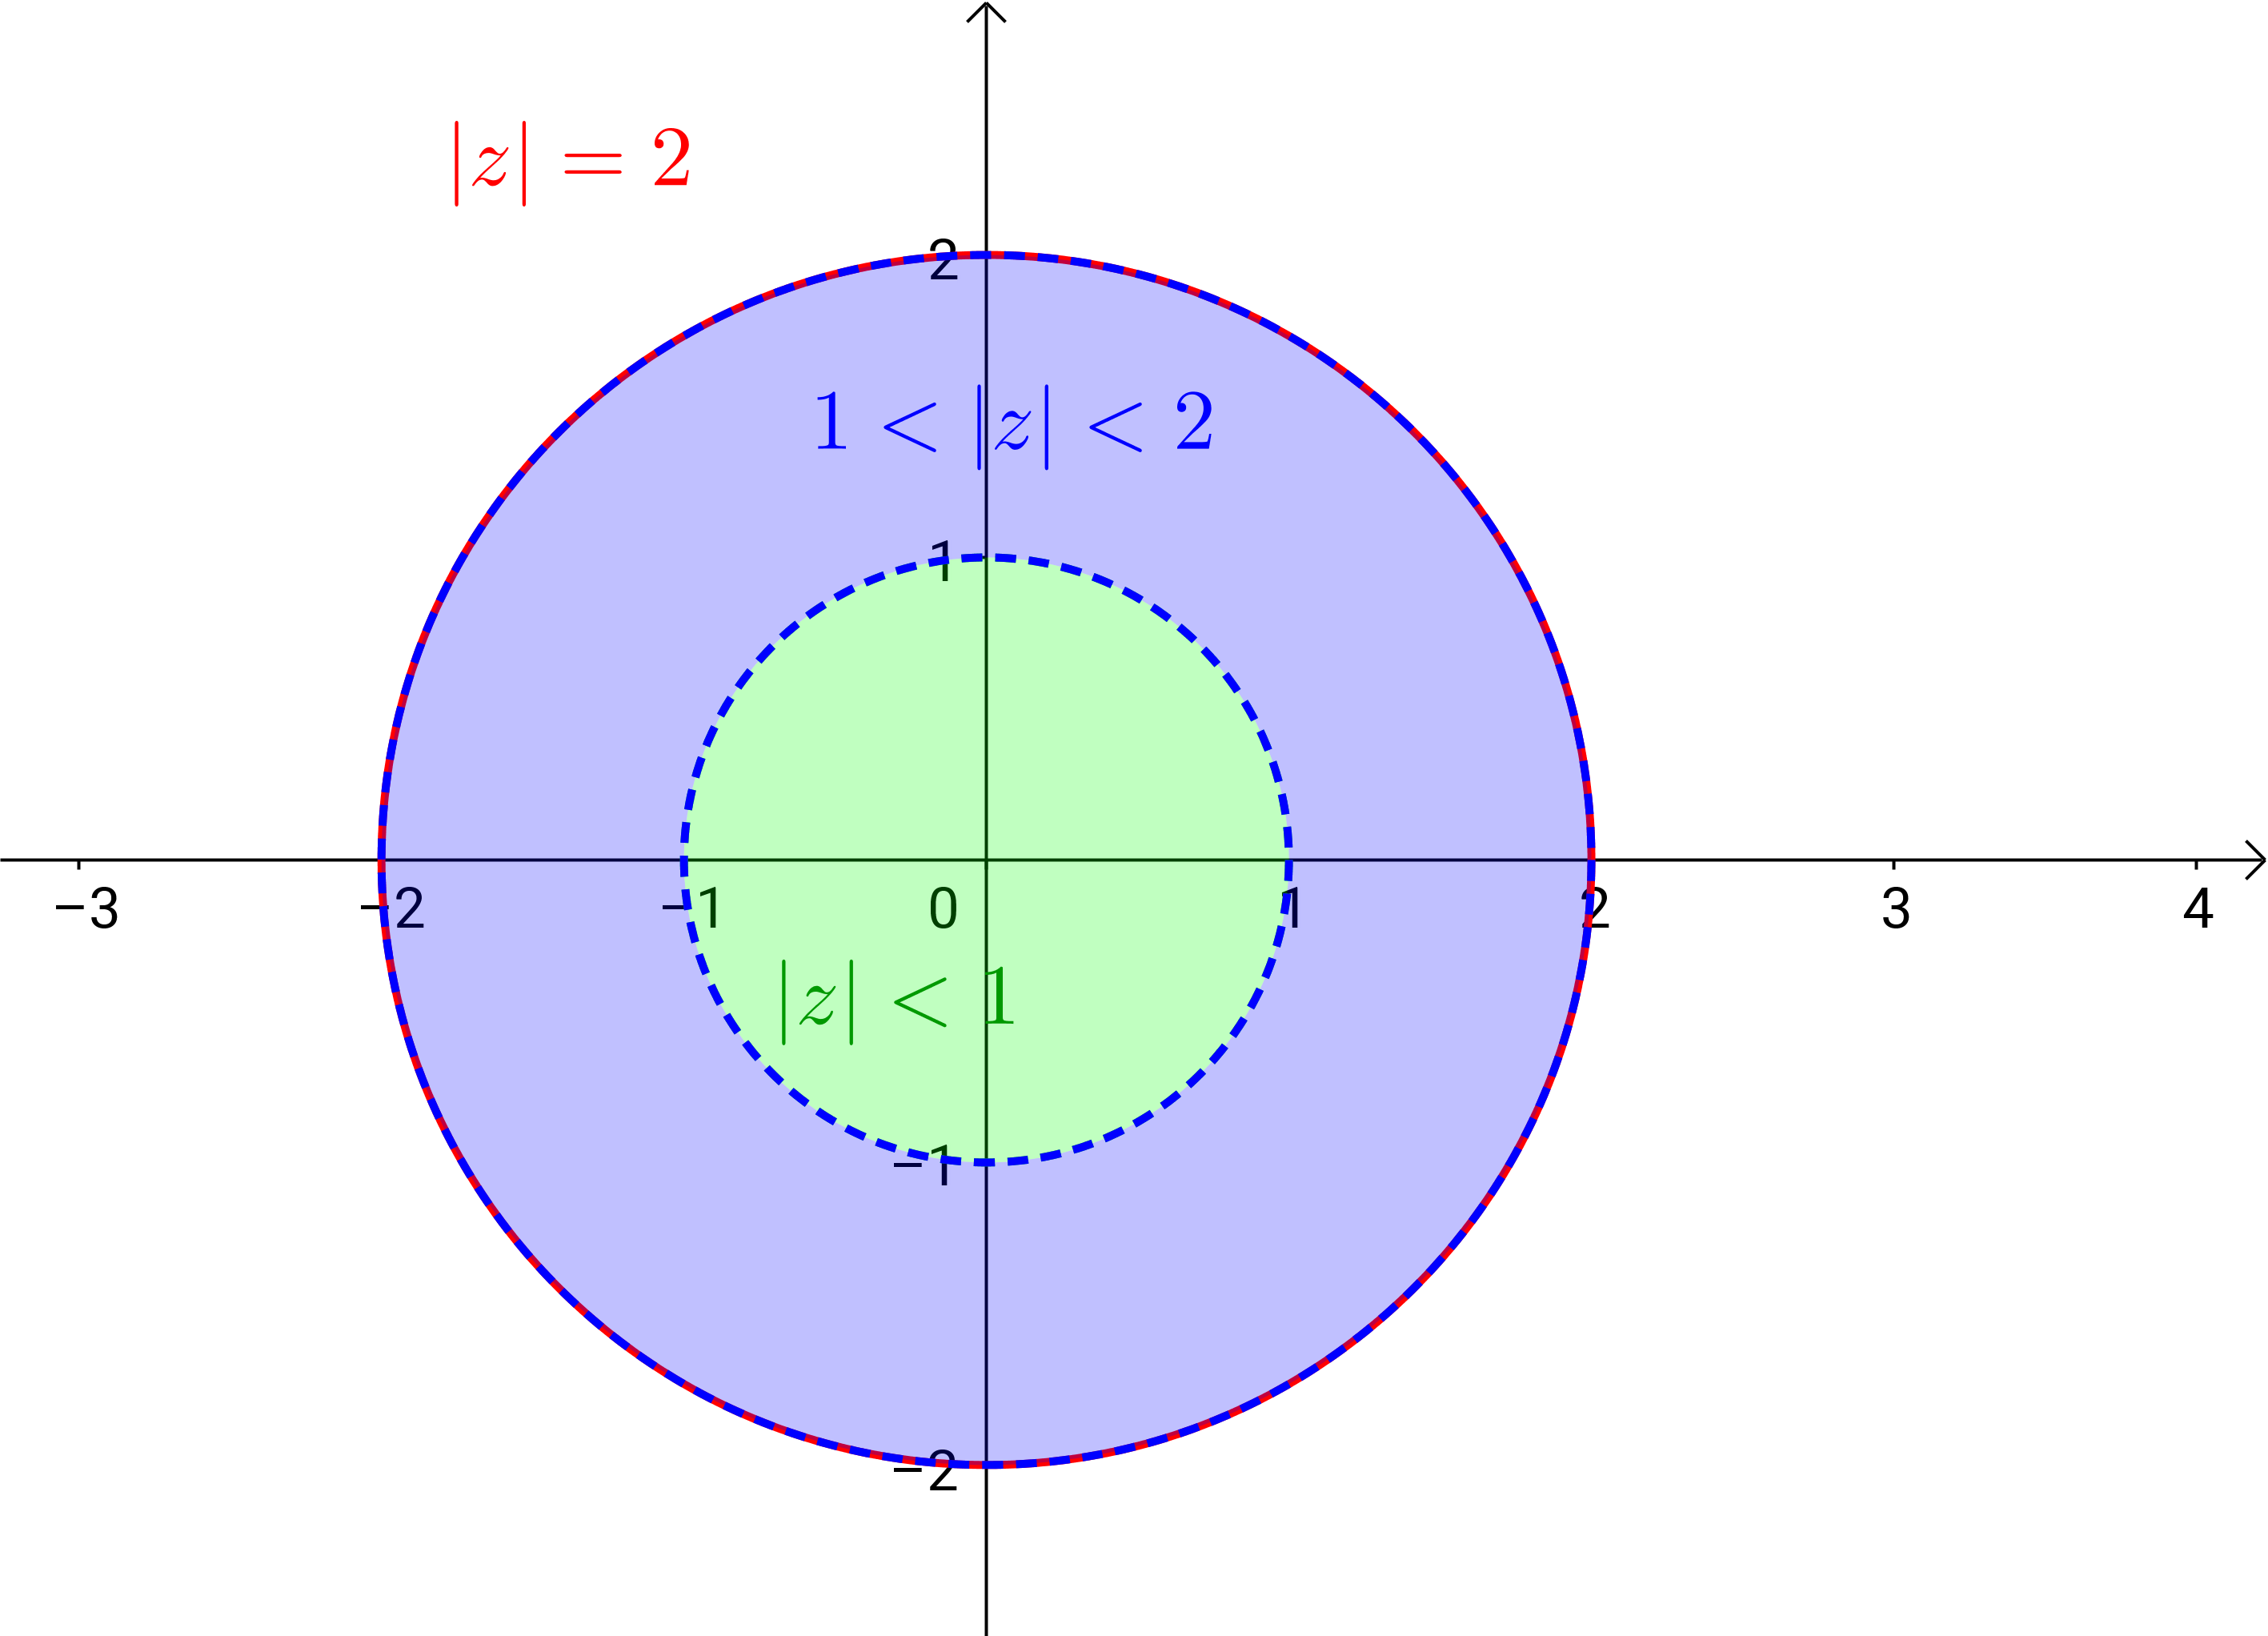
\includegraphics[width=.9\linewidth]{./img/opgave_3.png}
\caption{\label{opg3}Opgave 3}
\end{figure}

\section*{Opgave 4}
\label{sec:org95f5f49}

\subsection*{1. Benyt de Moivres formel med \(n=4\) til at bevise at}
\label{sec:orgf46108e}

$$\cos(4 \theta) = 8\cos^4(\theta) - 8 \cos^2(\theta) +1$$

Benytter som sagt de Moivres formel til at skrive

$$\left(\cos(\theta) + i \sin(\theta)\right)^4 = \cos(4\theta) + i \sin(4 \theta)\,.$$

Parentesen ophæves ved at multiplicere ud,

\begin{align*}
    \left(\cos(\theta) + i \sin(\theta)\right)^4 = &\cos^4(\theta) + 4 \cos^3(\theta) i \sin(\theta) + 6 \cos^2(\theta) i^2 \sin^2(\theta) \\
    &+ 4 \cos(\theta) i^3 \sin^3(\theta) +i^4 \sin^4(\theta) \\
    \left(\cos(\theta) + i \sin(\theta)\right)^4 = &\cos^4(\theta) + 4 \cos^3(\theta) i \sin(\theta) - 6 \cos^2(\theta) \sin^2(\theta) \\
    &- 4 \cos(\theta) i \sin^3(\theta) + \sin^4(\theta) 
\end{align*}

Det vides nu at

\begin{align*}
    \cos(4\theta) + i \sin(4\theta) = &\cos^4(\theta) + 4 \cos^3(\theta) i \sin(\theta) - 6 \cos^2(\theta) \sin^2(\theta) \\
    &- 4 \cos(\theta) i \sin^3(\theta) + \sin^4(\theta) 
\end{align*}

Ser nu kun på den reelle del

\begin{align*}
    \cos(4\theta) &= \cos^4(\theta) -6 \cos^2(\theta) \sin^2(\theta) + \sin^4(\theta)
\end{align*}

Udnytter at \(\sin^2(\theta) + \cos^2(\theta) =1 \to \sin^2(\theta) = 1 - \cos^2(\theta)\).

\begin{align*}
    \cos(4\theta) &= \cos^4(\theta) -6 \cos^2(\theta) \left(1 - \cos^2(\theta)\right) + \left(1 - \cos^2(\theta)\right)^2 \\
    \cos(4\theta) &= \cos^4(\theta) -6 \cos^2(\theta)  + 6\cos^4(\theta) + 1 +\cos^4(\theta) -2\cos^2(\theta)\\
    \cos(4\theta) &= 8\cos^4(\theta) -8 \cos^2(\theta)  + 1 \quad \triangle
\end{align*}

\subsection*{2. og udled at}
\label{sec:orge51d93d}

$$\cos\left(\frac{\pi}{8}\right) = \left(\frac{2 + \sqrt{2}}{4}\right)^{\frac{1}{2}}\,.$$

\(\frac{\pi}{8}\) indsættes i første omgang på \(\theta\)'s plads.

\begin{align*}
    \cos(4\theta) &= 8\cos^4(\theta) -8 \cos^2(\theta)  + 1\\
    \cos\left(4\cdot \frac{\pi}{8}\right) &= 8\cos^4\left(\frac{\pi}{8}\right) -8 \cos^2\left(\frac{\pi}{8}\right)  + 1 \\
    0 &= 8\cos^4\left(\frac{\pi}{8}\right) -8 \cos^2\left(\frac{\pi}{8}\right)  + 1 \quad , \, \cos\left(\frac{\pi}{2}\right) =0
\end{align*}

Nu indføres der en midlertidlig variabel \(w=\cos^2\left(\frac{\pi}{8}\right)\), så ligningen bliver til

$$0 = 8 w^2 -8w +1 \,.$$

Nu er der tale om en andengradsligning, som let løses:

\begin{align*}
    a &= 8 \\
    b &= -8 \\
    c &= 1 \\
    d &= b^2 - 4 a c \\
    d &= (-8)^2 - 4 \cdot 8 \cdot 1 = 32 \\
    w &= \frac{ -b \pm \sqrt{d}}{2 a} \\
    w &= \frac{ 8 \pm \sqrt{32}}{2 \cdot 8} \\
    w &= \frac{ 8 \pm \sqrt{32}}{16} \\
    w &= \frac{ 2 \pm \frac{\sqrt{32}}{4}}{4} \\
    w &= \frac{ 2 \pm \frac{\sqrt{32}}{\sqrt{16}}}{4} \\
    w &= \frac{ 2 \pm \sqrt{\frac{32}{16}}}{4} \\
    w &= \frac{ 2 \pm \sqrt{2}}{4} 
\end{align*}

Nu kan udtrykket for \(w\) sættes tilbage ind

\begin{align*}
    \cos^2\left(\frac{\pi}{8}\right) = \frac{ 2 \pm \sqrt{2}}{4}   \to \\
    \cos\left(\frac{\pi}{8}\right) = \pm \left(\frac{ 2 \pm \sqrt{2}}{4}\right)^\frac{1}{2}
\end{align*}

Af dette kan det ses at 

$$\cos\left(\frac{\pi}{8}\right) = \left(\frac{2 + \sqrt{2}}{4}\right)^{\frac{1}{2}}\,.$$

er indeholdt i løsningen. \(\triangle\)


\section*{Opgave 5}
\label{sec:org8b0605e}

\subsection*{1. Udtryk \(\sin^4(\theta)\) kun ved hjælp af trigonometriske funktioner med multiplum af vinkler (læs \(\sin(n\theta)\) eller \(\cos(n\theta)\).}
\label{sec:org596cd01}

Benytter i første omgang ligning (3.11):

\begin{align*}
    z - \frac{1}{z} = 2 i \sin(\theta) \to \\
    \left(z - \frac{1}{z}\right)^4 = \left(2 i \sin(\theta)\right)^4  \\
    \left(z - \frac{1}{z}\right)^4 = 2^4 i^4 \sin^4(\theta)  \\
    \left(z - \frac{1}{z}\right)^4 = 16 \sin^4(\theta)  \\
    z^4 + \frac{1}{z^4} -4 \cdot z^2 - 4 \cdot \frac{1}{z^2} + 6 = 16 \sin^4(\theta)  \\
    z^4 + \frac{1}{z^4} -4 \cdot \left(z^2 + \frac{1}{z^2}\right) + 6 = 16 \sin^4(\theta)
\end{align*}

Benytter nu ligning (3.6) til omskrivning

\begin{align*}
    2 \cos(4 \theta) - 4 \cdot 2 \cos(2\theta) + 6 = 16 \sin^4(\theta) \to \\
    \frac{2 \cos(4 \theta) - 4 \cdot 2 \cos(2\theta) + 6}{16} = \sin^4(\theta) \\
    \frac{1}{8} \cos(4 \theta) - \frac{1}{2} \cos(2\theta) + \frac{3}{8} = \sin^4(\theta) \quad \triangle
\end{align*}

\subsection*{2. Eftervis at den gennemsnitslige værdi over en periode er \(\frac{3}{8}\).}
\label{sec:orgf9061d0}

Den gennemsnitslige værdi findes ved at udføre følgende integrale

\begin{align*}
    \frac{\int_0^{2 \pi} \sin^4(\theta) d \theta}{2 \pi} &= \frac{\int_0^{2 \pi} \frac{1}{8} \cos(4 \theta) - \frac{1}{2} \cos(2\theta) + \frac{3}{8} \, d \theta}{2 \pi} \\
    \frac{\int_0^{2 \pi} \sin^4(\theta) d \theta}{2 \pi} &= \frac{\frac{1}{8}\int_0^{2 \pi}  \cos(4 \theta)\, d \theta  - \frac{1}{2}\int_0^{2 \pi}  \cos(2\theta)\, d \theta + \int_0^{2 \pi} \frac{3}{8} \, d \theta}{2 \pi} \\
    \frac{\int_0^{2 \pi} \sin^4(\theta) d \theta}{2 \pi} &= \frac{\frac{1}{8}\left[\frac{\sin(4\theta)}{4}\right]_0^{2 \pi} - \frac{1}{2}\left[  \frac{\sin(2\theta)}{2}\right]_0^{2 \pi} + \left[\frac{3}{8}\cdot \theta\right]_0^{2\pi}}{2\pi} \\
    \frac{\int_0^{2 \pi} \sin^4(\theta) d \theta}{2 \pi} &= \frac{\frac{1}{8}\left(\frac{\sin(8\cdot \pi)}{4}- \frac{\sin(0)}{4}\right) - \frac{1}{2}\left(  \frac{\sin(4\pi)}{2}-\frac{\sin(0)}{2}\right) + \left(\frac{3}{8}\cdot 2 \pi-\frac{3}{8}\cdot 0\right)}{2\pi} \\
    \frac{\int_0^{2 \pi} \sin^4(\theta) d \theta}{2 \pi} &= \frac{\frac{1}{8}\left(0-0 \right) - \frac{1}{2}\left(  0-0\right) + \left(\frac{3}{8}\cdot 2 \pi- 0\right)}{2\pi} \\
    \frac{\int_0^{2 \pi} \sin^4(\theta) d \theta}{2 \pi} &= \frac{\frac{3}{8} \cdot 2 \pi}{2 \pi} \\
    \frac{\int_0^{2 \pi} \sin^4(\theta) d \theta}{2 \pi} &= \frac{3}{8}  
\end{align*}

Hermed er det vist, at gennemsnittet over en periode er \(\frac{3}{8}\) \(\triangle\)

\section*{Opgave 6}
\label{sec:orgd0e58f0}

Find samtlige løsninger til følgende ligninger

\subsection*{1. \(x^3+8=0\)}
\label{sec:orga3514e3}

Benytter samme strategi som i eksemplerne i kapitel 3.3

\begin{align*}
    z^3 +8 &= 0 \to \\
    z^3 &= -8  \\
    z^3 &= -8\cdot 1  \\
    z^3 &= -8\cdot e^{2 \pi k i}\to  \\
    z &= \sqrt[3]{-8}\cdot e^{\frac{2 \pi k i}{3}}  \quad \text{ hvor } k=0,1,2 \\
    z &= -2\cdot e^{\frac{2 \pi k i}{3}}  \quad \text{ hvor } k=0,1,2 \\
    z_1 &= -2\cdot e^{\frac{2 \pi \cdot 0 \cdot  i}{3}}  \quad \text{ for } k=0 \\
    z_1 &= -2 \\
    z_2 &= -2 \cdot e^{\frac{2 \pi \cdot 1 \cdot  i}{3}}  \quad \text{ for } k=1 \\ 
    z_2 &= -2 \cdot \left( \cos\left(\frac{2\pi}{3}\right) + i \sin\left(\frac{2\pi}{3}\right)\right)\\ 
    z_2 &= -2 \cdot \left( -\frac{1}{2} + i \frac{\sqrt{3}}{2}\right)\\ 
    z_2 &= 1 + \sqrt{3}i \\
    z_3 &= -2 \cdot e^{\frac{4 \pi \cdot 1 \cdot  i}{3}}  \quad \text{ for } k=2 \\ 
    z_3 &= -2 \cdot \left( \cos\left(\frac{4\pi}{3}\right) + i \sin\left(\frac{4\pi}{3}\right)\right)\\ 
    z_3 &= -2 \cdot \left( -\frac{1}{2} - i \frac{\sqrt{3}}{2}\right)\\ 
    z_3 &= 1 - \sqrt{3}i 
\end{align*}

Ergo er der tre løsninger: \(z_1=-2\), \(z_2 = 1+\sqrt{3}i\) og \(z_3=1-\sqrt{3}i\).

\subsection*{2. \(z^4=16\)}
\label{sec:org14f9793}

Løses på tilsvarende vis som i forrige opgave:

\begin{align*}
    z^4 &= 16 \\
    z^4 &= 16 \cdot 1 \\
    z^4 &= 16 \cdot e^{2 \pi k i} \to \\
    z   &= \sqrt[4]{16} \cdot e^{\frac{2 \pi k i}{4}} \quad \text{ for } k=0,1,2,3 \\
    z   &= 2 \cdot e^{\frac{2 \pi k i}{4}} \quad \text{ for } k=0,1,2,3 \\
    z_1   &= 2 \cdot e^{\frac{2 \pi \cdot 0 \cdot i}{4}} \quad \text{ for } k=0 \\
    z_1   &= 2 \\
    z_2   &= 2 \cdot e^{\frac{2 \pi \cdot 1 \cdot i}{4}} \quad \text{ for } k=1 \\
    z_2   &= 2 \cdot \left(\cos\left(\frac{2 \pi \cdot 1 \cdot i}{4}\right) + i \sin\left(\frac{2 \pi \cdot 1 \cdot i}{4} \right) \right) \\
    z_2   &= 2 \cdot \left(0 + i 1 \right) \\
    z_2   &= 2i \\
    z_3   &= 2 \cdot e^{\frac{2 \pi \cdot 2 \cdot i}{4}} \quad \text{ for } k=2 \\
    z_3   &= 2 \cdot \left(\cos\left(\frac{2 \pi \cdot 2 \cdot i}{4}\right) + i \sin\left(\frac{2 \pi \cdot 2 \cdot i}{4} \right) \right) \\
    z_3   &= 2 \cdot \left(-1 + i 0 \right) \\
    z_3   &= -2 \\
    z_4   &= 2 \cdot e^{\frac{2 \pi \cdot 3 \cdot i}{4}} \quad \text{ for } k=3 \\
    z_4   &= 2 \cdot \left(\cos\left(\frac{2 \pi \cdot 3 \cdot i}{4}\right) + i \sin\left(\frac{2 \pi \cdot 3 \cdot i}{4} \right) \right) \\
    z_4   &= 2 \cdot \left(0 - i 1 \right) \\
    z_4   &= -2i 
\end{align*}

Ergo er der altså de fire løsninger \(z_1=2\), \(z_2=2i\), \(z_3=-2\) og \(z_4 = -2i\). \(\triangle\)

\subsection*{3. \(z^3 = 27 i\)}
\label{sec:org69ea70b}

I denne opgave udnyttes det at \(i=e^{i\left(\frac{\pi}{2}+2 \pi k \right)}\)

\begin{align*}
    z^3 &= 27 i \\
    z^3 &= 27 e^{i\left(\frac{\pi}{2}+2 \pi k \right)} \to\\
    z &= \sqrt[3]{27} e^{i\left(\frac{\frac{\pi}{2}+2 \pi k}{3} \right)} \quad \text{ for } k=0,1,2\\
    z &= 3 e^{i\left(\frac{\pi+4 \pi k}{6} \right)} \text{ for } k=0,1,2 \\
    z_1 &= 3 e^{i\left(\frac{\pi+4 \pi \cdot 0}{6} \right)}  \text{ for } k=0\\
    z_1 &= 3 e^{i\frac{\pi}{6}}  \\
    z_1 &= 3 \left( \cos\left(\frac{\pi}{6}\right) + i \sin\left(\frac{\pi}{6}\right)\right)  \\
    z_1 &= 3 \left( \frac{\sqrt{3}}{2} + i \frac{1}{2}\right)\\
    z_1 &= \frac{3}{2} \left( \sqrt{3} + i \right)\\
    z_2 &= 3 e^{i\left(\frac{\pi+4 \pi \cdot 1}{6} \right)}  \text{ for } k=1\\
    z_2 &= 3 \left( \cos\left(\frac{\pi+4 \pi \cdot 1}{6}\right) + i \sin\left(\frac{\pi+4 \pi \cdot 1}{6}\right)\right)  \\
    z_2 &= 3 \left( -\frac{\sqrt{3}}{2} + i \frac{1}{2}\right)\\
    z_2 &= \frac{3}{2} \left(- \sqrt{3} + i \right)\\
    z_3 &= 3 e^{i\left(\frac{\pi+4 \pi \cdot 1}{6} \right)}  \text{ for } k=2\\
    z_3 &= 3 \left( \cos\left(\frac{\pi+4 \pi \cdot 2}{6}\right) + i \sin\left(\frac{\pi+4 \pi \cdot 2}{6}\right)\right)  \\
    z_3 &= 3 \left( 0 - i \right)\\
    z_3 &= -3i
\end{align*}

Ergo er der altså de tre løsninger \(z_1=\frac{3}{2} \left(\sqrt{3} + i\right)\) ,\(z_2=\frac{3}{2} \left(-\sqrt{3} + i\right)\) og \(z_3 = -3i\). \(\triangle\)

\subsection*{4. \(z^3+z^2-2z =0\)}
\label{sec:org9e3ddb5}

I første omgang kan den trivielle løsning \(z_1=0\) let ses. Ligningen kan nu reduceres til:

$$z^2 + z -2 =0$$

Denne kan løses som en almindelig andengradsligning.

\begin{align*}
    a &= 1 \\
    b &= 1 \\
    c &= -2 \\
    d &= 1^2 - 4\cdot 1 \cdot (-2) = 9 \\
    z &= \frac{-1 \pm \sqrt{9}}{2 \cdot 1} \\
    z &= \frac{-1 \pm 3}{2 \cdot 1} \\
    z_2 &= 1 \\
    z_3 &= -2 
\end{align*}

Altså er der de tre løsninger \(z_1=0\), \(z_2=1\) og \(z_3=-2\).\(\triangle\)


\subsection*{5. \(z^3-2z^2 + 2z =0\)}
\label{sec:orge1972d0}

Igen ses den trivielle løsning \(z_1=0\) let, og ligningen kan reduceres til

$$z^2 -2z + 2 =0\,.$$

Løses igen som en almindelig andengradsligning:

\begin{align*}
    a &= 1 \\
    b &= -2 \\
    c &= 2 \\
    d &= (-2)^2-4\cdot 1\cdot 2 = 4 -8 = -4 \\
    z &= \frac{2 \pm \sqrt{-4}}{2 \cdot 1} \\
    z &= \frac{2 \pm 2i}{2 } \\
    z &= 1 \pm i \to \\
    z_2 &= 1 + i  \\
    z_3 &= 1 - i 
\end{align*}

Altså er der de tre løsninger \(z_1=0\), \(z_2 =1+i\) og \(z_3=1-i\).\(\triangle\)
\end{document}